\documentclass[11pt,chapterprefix=true,toc=bibliography,numbers=noendperiod,
               footnotes=multiple]{scrbook}
\usepackage{fixltx2e} % LaTeX patches, \textsubscript
\usepackage{microtype}
\usepackage{cmap} % fix search and cut-and-paste in Acrobat
\usepackage{ifthen}
\usepackage[oldstylenums,largesmallcaps]{kpfonts}
\usepackage[T1]{fontenc}
\usepackage[utf8]{inputenc}
\usepackage[british]{babel}
\usepackage{csquotes}
\usepackage{tabularx}
\usepackage{graphicx}
\usepackage{booktabs}
\usepackage{algorithmicx}
\usepackage{algpseudocode}
\usepackage{algorithm}
\usepackage{listings}
\usepackage[table,hyperref,dvipsnames]{xcolor}
\usepackage[hidelinks]{hyperref}
\usepackage[autocite=footnote,citestyle=authoryear-comp,bibstyle=authoryear,
            isbn=false,doi=false,backend=biber]{biblatex}
\usepackage{nag}

%%% Custom LaTeX preamble
% serif, non-bold headings:
\addtokomafont{chapter}{\mdseries}
\addtokomafont{disposition}{\rmfamily}
\addtokomafont{descriptionlabel}{\rmfamily}
\addtokomafont{pageheadfoot}{\itshape}
% section numbering up to subsection
\setcounter{secnumdepth}{2}
% hyperlinks
\urlstyle{same} % normal text font (alternatives: tt, rm, sf)
\hypersetup{
  pdftitle={Extending Raft with structured voting},
  pdfauthor={Leonhard Markert (lm510), Emmanuel College}
}
\addbibresource{Bibliography.bib}
\pagestyle{headings}
% custom commands
\newcommand{\requestVoteRPC}[0]{\texttt{requestVote} \textsc{rpc}}
\newcommand{\appendEntriesRPC}[0]{\texttt{appendEntries} \textsc{rpc}}
\newcommand{\voted}[1]{\textbf{\color{black}#1}}

%%% Body
\begin{document}

\frontmatter

\begin{titlepage}

\rightline{\large\textit{Leonhard Markert}} \medskip
\rightline{\large\textit{Emmanuel College}} \medskip
\rightline{\large\textit{lm510}}

\vfil

\centerline{\large Computer Science Part \textsc{ii} Project} \vspace{0.4in}
\centerline{\Large\textbf{Extending Raft with structured voting}} \vspace{0.3in}
\centerline{\large\textit{\today}}

\vfil

\begin{center}
{\renewcommand{\arraystretch}{2}%
\begin{tabularx}{316pt}{rX}
\textbf{Project Supervisors} & \textit{Malte Schwarzkopf} and \textit{Ionel Gog} \\
\textbf{Director of Studies} & \textit{Dr Jonathan Hayman} \\
\textbf{Overseers} & \textit{Dr Markus Kuhn} and \textit{Dr Neal Lathia}
\end{tabularx}}
\end{center}

\end{titlepage}

\chapter*{Proforma\label{ch:proforma}}

\begin{center}
{\renewcommand{\arraystretch}{1.5}%
\begin{tabularx}{330pt}{rX}
\textbf{Name and College} & Leonhard Markert, Emmanuel College \\
\textbf{Project Title} & Extending Raft with structured voting \\
\textbf{Examination} & Computer Science Tripos, Part \textsc{ii}, June 2014 \\
\textbf{Word Count} & XXX words \\
\textbf{Project Originator} & Leonhard Markert \\
\textbf{Project Supervisors} & Malte Schwarzkopf and Ionel Gog
\end{tabularx}}
\end{center}

\section*{Original aims of the project\label{sc:original-aims}}

XXX

\section*{Work completed\label{sc:work-completed}}

XXX

\section*{Special Difficulties\label{sc:special-difficulties}}

None.

\section*{Declaration of Originality\label{sc:declaration-of-originality}}

I, Leonhard Markert of Emmanuel College, being a candidate for Part~\textsc{ii} of the Computer Science Tripos, hereby declare that this dissertation and the work described in it are my own work, unaided except as may be specified below, and that the dissertation does not contain material that has already been used to any substantial extent for a comparable purpose.

\vspace{0.3in}
Signed

\vspace{0.2in}
Date \hspace{0.4in} \today

\chapter*{Acknowledgements\label{ch:acknowledgements}}

\begin{itemize}
    \item Malte Schwarzkopf and Ionel Gog
    \item Christian Storm
    \item Andrew Stone
\end{itemize}

\tableofcontents

\mainmatter

\chapter{Introduction\label{ch:introduction}}

% \begin{itemize}
    % \item Principal motivation for the project
    % \item How the work fits into the broad area of surrounding CS
    % \item Survey of related work
% \end{itemize}

% \begin{itemize}
    % \item Raft: consensus protocol, asymmetric: leader, follower, candidate -- elections, majority voting by default; state machine, backend, ``understandable'' Paxos replacement -- strongly consistent (all operations are seen in the same order by all nodes); correctness proof \parencite{raft} \parencite{raftproof}
    % \item Structured voting: more efficient / available (less cost), example: Grid protocol, key insight: don't need majority to guarantee mutual exclusion; tree-shaped voting structures: generalised framework; logical structure on nodes; smaller quorums
    % \item Motivation: combine Raft and structured voting (\textit{write} quorums specifically)
    % \item Failure model: no Byzantine failures -- servers either work or not; fail-stop, permanent/volatile memory, lost/delayed messages but not corrupted
% \end{itemize}

\section{Motivation\label{sc:motivation}}

As ever-increasing amounts of data are being handled in commercial settings as well as in research, distributed systems for processing and storage are becoming more and more ubiquitous. One main driver of this development is the need to increase fault tolerance.

According to Eric Brewer's famous \textsc{cap} theorem \autocite{cap}, a partition tolerant system cannot be both strictly consistent and maximally available.\footnote{The terms consistency, availability and partition tolerance are defined in \autoref{ssc:cap-acid-and-base}.} Many recent distributed data stores sacrifice consistency for availability. Some applications, however, require strong consistency guarantees -- data backup and configuration management systems, for example. Consensus protocols like Paxos \autocite{paxos} and Raft \autocite{raft} guarantee consistency at the cost of decreased availability.

In this project, I added support for structured voting schemes to an existing implementation of Raft. My aim was increase the availability and scalability of data storage systems built on top of this implementation while still providing the same consistency guarantees as the original Raft algorithm.

Increasing the availability of a consistent distributed system would have two effects:

\begin{itemize}
    \item Applications that require consistency and already use a consensus algorithm that provides consistency could have their availability increased by migrating to this new implementation;
    \item Applications that require high availability and currently run an algorithm that does not guarantee consistency, might switch to this new implementation too.
\end{itemize}

\section{Challenges\label{sc:challenges}}

\section{Related work\label{sc:related-work}}

\subsection{Distributed systems: \textsc{cap}, \textsc{acid} and \textsc{base}\label{ssc:cap-acid-and-base}}

Eric Brewer's famous \textsc{cap} theorem states that any distributed system can provide at most two out of the three desirable properties consistency (\textsc{c}), availability (\textsc{a}), and partition tolerance (\textsc{p}).\autocite{cap} The following definitions are adapted from \textcite{capproof}:

\begin{description}
    \item[Consistency] There must exist a total order on all operations such that each operation looks as if it were completed at a single instant. An important consequence of this \emph{linearisable} (or \emph{atomic}) consistency guarantee is that any read operation that begins after a write operation completes must return that value, or the result of a later write operation.\footnote{As \textcite{capproof} point out, the term \emph{consistency} is highly overloaded. Note that the above notion of atomic consistency subsumes what is called atomicity and consistency in the context of \textsc{acid} (\enquote{atomic, consistent, isolated, durable}) databases.}
    \item[Availability] Every request received by a non-failing node in the system must result in a response.
    \item[Partition tolerance] The system continues to operate despite arbitrary message loss. This includes network partitions, where all messages sent from nodes in one component of the partition to nodes in another component are lost.
\end{description}

Out of those three, partition tolerance is required in almost all cases. As \citeauthor{needp} puts it in his article \citetitle{needp}:

\begin{quote}
    For a distributed \dots{} system to \emph{not} require partition tolerance it would have to run on a network which is guaranteed to never drop messages \dots{} and whose nodes are guaranteed to never [fail]. [These] types of systems \dots{} don't exist.
\end{quote}

This leaves designers of distributed systems with the task of finding the right trade-off between consistency and availability, both of which should be considered as continuous rather than binary properties \autocite{cap12}. With the rise of commercial databases of unprecedented scale over the last decade, consistency (in its strict form as defined above) is in many cases sacrificed for increased availability.%
\footnote{This has been heralded as a paradigm shift from the \textsc{acid} to the \textsc{base} (\enquote{basically available, soft state, eventually consistent}) model \parencite{base}.} %
The authors of \citetitle{dynamo} describe this as follows:%
\footnote{Notable other eventually consistent systems include Cassandra \parentext{\citeurl{cassandra}}, Riak \parentext{\citeurl{riak}} and HBase \parentext{\citeurl{hbase}}.}

\begin{quote}
    For systems prone to server and network failures, availability can be increased by using optimistic replication techniques, where changes are allowed to propagate to replicas in the background, and concurrent, disconnected work is tolerated. The challenge with this approach is that it can lead to \emph{conflicting changes which must be detected and resolved} \dots{} Dynamo is designed to be an eventually consistent data store; that is all updates reach all replicas eventually.
\end{quote}

The conflict detection and resolution mechanisms required by eventually consistent systems increase their complexity compared to consistent systems, which do not need them. This begs the question: are there techniques that could be used to improve availability without giving up on consistency, allowing for simpler systems? The \textsc{cap} theorem tells us that we can never build strictly consistent and maximally available systems, but a different trade-off might be possible.

\subsection{The Raft consensus algorithm\label{ssc:raft-consensus-algorithm}}

Although still a draft, the paper describing the new Raft consensus algorithm \autocite{raft} has created a lot of buzz; dozens of implementations in various languages and stages of development already exist.\footnote{For an up-to-date list of Raft implementations, see \url{http://raftconsensus.github.io/\#implementations}.}

In the following, I will give a short overview of the Raft consensus algorithm. It is meant to introduce the terminology required for the Implementation and Evaluation chapters.

At its core, Raft uses a replicated state machine architecture, implemented using a replicated log (see \autoref{fig:replicated-state-machine}): each log contains the same commands in the same order, so each state machine processes the same sequence of commands. Since the state machines are assumed to be deterministic, each computes the same state and the same sequence of outputs.

\begin{figure}[h]
    \centering
    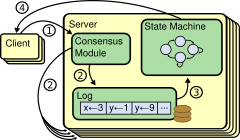
\includegraphics[width=0.5\textwidth, keepaspectratio]{Images/Replicated_state_machine.pdf}
    \caption{Replicated state machine architecture}
    \label{fig:replicated-state-machine}
\end{figure}

Raft implements this replicated log architecture using a collections of servers (a cluster) communicating via remote procedure calls (\textsc{rpc}s), of which there are two: \texttt{appendEntries} and \texttt{requestVote}. At any given time each server is either a \emph{leader}, \emph{follower}, or \emph{candidate} (see \autoref{fig:consensus-fsm}). In normal operation, there is exactly one leader and all other servers are followers.

\begin{figure}[h]
    \centering
    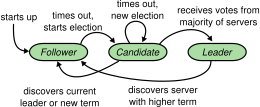
\includegraphics[width=0.5\textwidth, keepaspectratio]{Images/Consensus_FSM.pdf}
    \caption{Server states and the transitions between them}
    \label{fig:consensus-fsm}
\end{figure}

\minisec{Leader election}

A server remains in follower state as long as it receives valid heartbeats (\appendEntriesRPC s that carry no entries) from a leader or candidate. If a follower receives no communication over a period of time, it assumes that there is no viable leader and begins an election to choose a new one. To do so, it transitions to candidate state and issues \requestVoteRPC s in parallel to all other servers in the cluster. Then one of three things happens: (a) the candidate wins the election, (b) another server establishes itself as leader, or (c) a period of time goes by without a winner, in which case a new election is started.

Each server receiving a \requestVoteRPC{} will vote for at most one candidate, on a first-come-first-served basis. Once a candidate wins an election, it becomes the new leader and sends heartbeat messages to every other server to establish its authority.

\minisec{Log replication}

Each client request to a leader contains a command to be executed by the replicated state machines. The leader appends the command to its log as a new entry, then issues \appendEntriesRPC s in parallel to all other servers to replicate the entry. When the entry has been safely replicated, the leader applies the entry to its state machine and returns the result of that execution to the client (for a complete description of what it means for an entry to be \enquote{safely replicated}, see subsection 5.3 of the Raft paper.)

\minisec{Safety guarantees}

In order to guarantee overall correctness, different components of Raft are designed to make sure certain well-defined safety properties are true at all times. These properties are shown to hold and then used to prove correctness in the separate correctness proof \autocite{raftproof}.

Since my project involved changing the way in which quorums\footnote{A \emph{quorum} is a minimal subset of the cluster that an operation has to obtain votes from in order to be performed. Majority voting, for example, specifies that any set of servers containing at least half the servers in the entire cluster constitutes a quorum.} are constructed, I had to pay special attention to the Election Safety property (stating that there can be at most one leader at any given time) and all the steps in the proof to do with quorums, in order to make sure all the desired properties still hold.

\subsection{Structured voting schemes\label{ssc:structured-voting-schemes}}

By taking into account the identity of nodes, as opposed to just counting them as in the majority consensus algorithm, we can build \emph{structured} voting schemes.

\minisec{Quorum systems}

A quorum system is defined as a tuple of a read and a write quorum set whose elements are called read quorums and write quorums, respectively. These are constructed such that every write quorum intersects with every other write quorum and with every read quorum in at least one process while read quorums need not intersect \autocite{voting}.

The key realisation that lead to this project was that write quorums have precisely the property required for Raft's leader election, namely that any two write quorums intersect. From this point on, \emph{quorum} will mean \emph{write quorum} unless specifically noted otherwise.

\minisec{Structured voting by example}

Structured voting schemes impose a logical structure on the set of processes and use structural properties to specify quorum systems. For example, the structured Grid Protocol arranges processes in a logical rectangular grid \autocite{grid}. A write quorum consists of all processes from a complete column plus one process from each column.

\begin{figure}[h]
    \centering
    {\ttfamily\color{gray}
    \begin{tabular}{c | c | c | c}
        A & \voted{B} & C & D \\
        \hline
        E & \voted{F} & \voted{G} & H \\
        \hline
        \voted{I} & \voted{J} & K & L \\
        \hline
        M & \voted{N} & O & \voted{P} \\
    \end{tabular}
    }
    \caption{A Grid Protocol quorum: The entire second column (\texttt{B}, \texttt{F}, \texttt{J}, \texttt{N}) and one process from each other column (\texttt{I}, \texttt{G}, \texttt{P}) are included}
    \label{fig:grid-quorum}
\end{figure}

\minisec{Specifying voting structures}

\citeauthor{generators} present \emph{tree-shaped voting structures} as a universal quorum system representation in the form of semantics-enriched tree graphs. They are produced by voting structure specific \emph{voting structure generators} \autocite{generators}.

In a tree-shaped voting structure, each node without children (a \enquote{physical node}) represents a process. Nodes with children (called \enquote{virtual nodes}) do not stand for processes. Instead, they represent the structure of the voting scheme. The tree is to be interpreted such that votes flow upwards, from the physical nodes (the leaves of the tree) up to the virtual node at its root.

When a physical node casts its vote, the number of votes it is annotated with is added to the votes its parent virtual node has received. If the sum of those votes equals or exceeds the parent node's threshold, then the parent node in turn passes its vote to its parent. An annotated example is given in \autoref{fig:grid4}.

\begin{figure}[h]
    \centering
    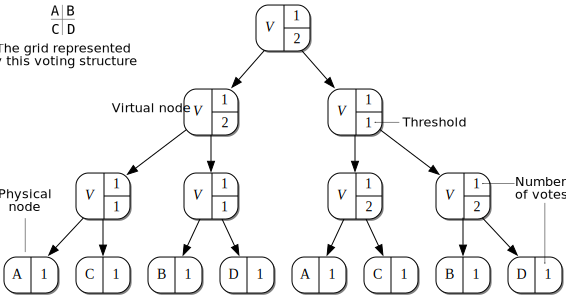
\includegraphics[width=0.8\textwidth, keepaspectratio]{Images/Grid4.pdf}
    \caption{A tree-structured voting scheme for a Grid Protocol managing four processes \texttt{A}, \texttt{B}, \texttt{C} and \texttt{D}.}
    \label{fig:grid4}
\end{figure}


\section{Overview of Structured Rafter\label{sc:overview-of-structured-rafter}}

\chapter{Preparation\label{ch:preparation}}

% \begin{itemize}
    % \item Work undertaken before code was written
    % \item Refinement of project proposal
    % \item Professional approach: Requirements analysis!, reference Software Engineering techniques
    % \item PLs and systems which had to be learnt, theories and algorithms which required understanding
% \end{itemize}

\chapter{Implementation\label{ch:implementation}}

% \begin{itemize}
    % \item Describe what was actually produced
    % \item Design strategies (looking ahead to the testing stage)
    % \item Draw attention to the parts of the work which are not your own
    % \item Mention major milestones
% \end{itemize}

\chapter{Evaluation\label{ch:evaluation}}

% \begin{itemize}
    % \item Signs of success, evidence of thorough and systematic testing
    % \item Sample output, graphs, diagrams
    % \item Original goals achieved? Proof? Did stuff work?
% \end{itemize}

% \begin{itemize}
    % \item Failure modes presentation: most frequent failure modes are individual, then rack failures
% \end{itemize}

\chapter{Conclusions\label{ch:conclusions}}

% \begin{itemize}
    % \item Refer to Introduction
    % \item Lessons learnt
% \end{itemize}

\printbibliography

\backmatter

\appendix

\chapter{Code samples\label{ch:code-samples}}

\end{document}
